%% BioMed_Central_Tex_Template_v1.06
%%                                      %
%  bmc_article.tex            ver: 1.06 %
%                                       %

%%IMPORTANT: do not delete the first line of this template
%%It must be present to enable the BMC Submission system to
%%recognise this template!!

%%%%%%%%%%%%%%%%%%%%%%%%%%%%%%%%%%%%%%%%%
%%                                     %%
%%  LaTeX template for BioMed Central  %%
%%     journal article submissions     %%
%%                                     %%
%%          <8 June 2012>              %%
%%                                     %%
%%                                     %%
%%%%%%%%%%%%%%%%%%%%%%%%%%%%%%%%%%%%%%%%%


%%%%%%%%%%%%%%%%%%%%%%%%%%%%%%%%%%%%%%%%%%%%%%%%%%%%%%%%%%%%%%%%%%%%%
%%                                                                 %%
%% For instructions on how to fill out this Tex template           %%
%% document please refer to Readme.html and the instructions for   %%
%% authors page on the biomed central website                      %%
%% http://www.biomedcentral.com/info/authors/                      %%
%%                                                                 %%
%% Please do not use \input{...} to include other tex files.       %%
%% Submit your LaTeX manuscript as one .tex document.              %%
%%                                                                 %%
%% All additional figures and files should be attached             %%
%% separately and not embedded in the \TeX\ document itself.       %%
%%                                                                 %%
%% BioMed Central currently use the MikTex distribution of         %%
%% TeX for Windows) of TeX and LaTeX.  This is available from      %%
%% http://www.miktex.org                                           %%
%%                                                                 %%
%%%%%%%%%%%%%%%%%%%%%%%%%%%%%%%%%%%%%%%%%%%%%%%%%%%%%%%%%%%%%%%%%%%%%

%%% additional documentclass options:
%  [doublespacing]
%  [linenumbers]   - put the line numbers on margins

%%% loading packages, author definitions

%\documentclass[twocolumn]{bmcart}% uncomment this for twocolumn layout and comment line below
\documentclass{bmcart}

%%% Load packages
\usepackage{amsthm,amsmath}
\usepackage{url}
\usepackage{float}
\usepackage{graphicx}

%\RequirePackage{natbib}
%\RequirePackage[authoryear]{natbib}% uncomment this for author-year bibliography
%\RequirePackage{hyperref}
\usepackage[utf8]{inputenc} %unicode support
%\usepackage[applemac]{inputenc} %applemac support if unicode package fails
%\usepackage[latin1]{inputenc} %UNIX support if unicode package fails


%%%%%%%%%%%%%%%%%%%%%%%%%%%%%%%%%%%%%%%%%%%%%%%%%
%%                                             %%
%%  If you wish to display your graphics for   %%
%%  your own use using includegraphic or       %%
%%  includegraphics, then comment out the      %%
%%  following two lines of code.               %%
%%  NB: These line *must* be included when     %%
%%  submitting to BMC.                         %%
%%  All figure files must be submitted as      %%
%%  separate graphics through the BMC          %%
%%  submission process, not included in the    %%
%%  submitted article.                         %%
%%                                             %%
%%%%%%%%%%%%%%%%%%%%%%%%%%%%%%%%%%%%%%%%%%%%%%%%%


%\def\includegraphic{}
%\def\includegraphics{}



%%% Put your definitions there:
\startlocaldefs
\endlocaldefs

\newcommand{\noun}[1]{\textsc{#1}}
\floatstyle{ruled}
\newfloat{algorithm}{tbp}{loa}
\providecommand{\algorithmname}{Algorithm}
\floatname{algorithm}{\protect\algorithmname}


%%% Begin ...
\begin{document}

%%% Start of article front matter
\begin{frontmatter}

\begin{fmbox}
\dochead{Research}

%%%%%%%%%%%%%%%%%%%%%%%%%%%%%%%%%%%%%%%%%%%%%%
%%                                          %%
%% Enter the title of your article here     %%
%%                                          %%
%%%%%%%%%%%%%%%%%%%%%%%%%%%%%%%%%%%%%%%%%%%%%%

\title{Using Bayesian networks to predict some regulatory systems components of Escherichia coli from microarray gene expression data}

%%%%%%%%%%%%%%%%%%%%%%%%%%%%%%%%%%%%%%%%%%%%%%
%%                                          %%
%% Enter the authors here                   %%
%%                                          %%
%% Specify information, if available,       %%
%% in the form:                             %%
%%   <key>={<id1>,<id2>}                    %%
%%   <key>=                                 %%
%% Comment or delete the keys which are     %%
%% not used. Repeat \author command as much %%
%% as required.                             %%
%%                                          %%
%%%%%%%%%%%%%%%%%%%%%%%%%%%%%%%%%%%%%%%%%%%%%%

\author[
   addressref={univalle},                   % id's of addresses, e.g. {aff1,aff2}
   corref={univalle},                       % id of corresponding address, if any
   %noteref={n1},                        % id's of article notes, if any
   email={digarjim@hotmail.com}   % email address
]{\inits{DG}\fnm{Diego M} \snm{García}}
\author[
   addressref={univalle},
   email={irenetischer@gmail.com}
]{\inits{IT}\fnm{Irene} \snm{Tischer}}

%%%%%%%%%%%%%%%%%%%%%%%%%%%%%%%%%%%%%%%%%%%%%%
%%                                          %%
%% Enter the authors' addresses here        %%
%%                                          %%
%% Repeat \address commands as much as      %%
%% required.                                %%
%%                                          %%
%%%%%%%%%%%%%%%%%%%%%%%%%%%%%%%%%%%%%%%%%%%%%%

\address[id=univalle]{%                           % unique id
  \orgname{EISC, Universidad del Valle}, % university, etc
  \street{Calle 13 No. 100-00},                     %
  %\postcode{}                                % post or zip code
  \city{Cali},                              % city
  \cny{Colombia}                                    % country
}

%%%%%%%%%%%%%%%%%%%%%%%%%%%%%%%%%%%%%%%%%%%%%%
%%                                          %%
%% Enter short notes here                   %%
%%                                          %%
%% Short notes will be after addresses      %%
%% on first page.                           %%
%%                                          %%
%%%%%%%%%%%%%%%%%%%%%%%%%%%%%%%%%%%%%%%%%%%%%%

\begin{artnotes}
%\note{Sample of title note}     % note to the article
\note[id=n1]{Equal contributor} % note, connected to author
\end{artnotes}

\end{fmbox}% comment this for two column layout

%%%%%%%%%%%%%%%%%%%%%%%%%%%%%%%%%%%%%%%%%%%%%%
%%                                          %%
%% The Abstract begins here                 %%
%%                                          %%
%% Please refer to the Instructions for     %%
%% authors on http://www.biomedcentral.com  %%
%% and include the section headings         %%
%% accordingly for your article type.       %%
%%                                          %%
%%%%%%%%%%%%%%%%%%%%%%%%%%%%%%%%%%%%%%%%%%%%%%

\begin{abstractbox}

\begin{abstract} % abstract
Identification and analysis of signature genes and its interactions are keys on pharmacist design process, improve physiological of plants and research of disease as oncogenesis, among others. it is possible to analyze the collective behavior of genes using models that represent the interaction between them. Some of these models are gene co-expression networks and gene regulatory networks; where we can observe the expression patterns that follow gene groups under given biological conditions and the impact of the behavior of one group of genes over other. The networks in question have been represented with models like Bayesian network and we can infer its structure and parameters using statistical methods like Markov Chain Monte Carlo simulation (MCMC) and Bayesian inference. 

Purpose of this work is to valid the useful of Bayesian networks to predict several bacterial regulatory system components: First, we obtain gene expression data of 4297 genes of Escherichia coli and 466 observations in several biological conditions. Selection genes process was done using gene coexpression networks and identifying signature genes across of caracterization of modules to functional level and topological, so we use a subset of modular genes and then discretize the data into three categories. Second, we learned Bayesian networks of gene interactions adopting MCMC simulation and Bayesian inference methods. Specifically, we use Metropolis Hasting algorithm and Posterior distribution to approximate the parameters and structure of network. To avoid overfitting in the learning we include two constraints during simulations: maximum in-grade in nodes and minimum dependence in edges of network. Third, we compare the genes interactions that we found with some published on ABASY for modular genes in bacterial regulatory systems specifically, Escherichia coli. Finally, we found Bayesian networks that correspond to components of modular genes like lactose, sodium ion transport and phosphorelay signal transduction system in Escherichia coli.

In this work, we see that Bayesian networks can help us to understand some bacterial regulatory systems components, mainly components of modular genes, however, only its learning method from microarray gene expression data can\textquoteright t say us about other components such as global regulators, inter-modular regulators and basal machinery.
\end{abstract}

%%%%%%%%%%%%%%%%%%%%%%%%%%%%%%%%%%%%%%%%%%%%%%
%%                                          %%
%% The keywords begin here                  %%
%%                                          %%
%% Put each keyword in separate \kwd{}.     %%
%%                                          %%
%%%%%%%%%%%%%%%%%%%%%%%%%%%%%%%%%%%%%%%%%%%%%%

\begin{keyword}
\kwd{Bayesian networks}
\kwd{MCMC simulation}
\kwd{complex network analysis}
\kwd{microarrays}
\kwd{bacterial regulatory systems}
\end{keyword}

% MSC classifications codes, if any
%\begin{keyword}[class=AMS]
%\kwd[Primary ]{}
%\kwd{}
%\kwd[; secondary ]{}
%\end{keyword}

\end{abstractbox}
%
%\end{fmbox}% uncomment this for twcolumn layout

\end{frontmatter}

%%%%%%%%%%%%%%%%%%%%%%%%%%%%%%%%%%%%%%%%%%%%%%
%%                                          %%
%% The Main Body begins here                %%
%%                                          %%
%% Please refer to the instructions for     %%
%% authors on:                              %%
%% http://www.biomedcentral.com/info/authors%%
%% and include the section headings         %%
%% accordingly for your article type.       %%
%%                                          %%
%% See the Results and Discussion section   %%
%% for details on how to create sub-sections%%
%%                                          %%
%% use \cite{...} to cite references        %%
%%  \cite{koon} and                         %%
%%  \cite{oreg,khar,zvai,xjon,schn,pond}    %%
%%  \nocite{smith,marg,hunn,advi,koha,mouse}%%
%%                                          %%
%%%%%%%%%%%%%%%%%%%%%%%%%%%%%%%%%%%%%%%%%%%%%%

%%%%%%%%%%%%%%%%%%%%%%%%% start of article main body
% <put your article body there>

%%%%%%%%%%%%%%%%
%% Background %%
%%
\section*{Background}
\subsection*{Bayesian networks}
A Bayesian network is a directed acyclic graph (DAG), in which nodes represent random variables and edges denote dependencies between them (see \cite{Pearl:1988:PRI:52121,pmid23375235}).  Such graph can be defined as a pair $B=(G,\Theta)$; where $G=(V,E)$, $V$ denote a set of nodes, $E$ a set of edges and $\Theta$ a vector of conditional probabilities. We can say that $v_{p}$ is parent of $v_{i}$ for all $v_{c},v_{p}\in V$ with $c\neq p$ if there is an edge from $v_{p}$ to $v_{c}$. The set of all parents of $v_{i}$ will be denote $Pa(v_{i})$ and the joint distribution of the variables $V=\{\nu_{1},...,\nu_{d}\}$ can be specified by decomposition:
\begin{equation}
P(V)=\prod_{i=1}^{d}P(\nu_{i}|Pa(\nu_{i}))\label{eq:1}
\end{equation}
On the other hand, DNA microarrays are a technology that allows monitoring broad levels of gene expression for organism given; these experiments concurrently measure the expression level of thousands of genes. An improtant problem in computational biology is to discover, from such measurements, gene interaction networks and key biological features of cellular systems (see \cite{dey2010bayesian}). To learn a Bayesian networks from gene expression data is often used to address this problem (see \cite{Pearl:1988:PRI:52121}).\\
\\
Now, let $v_{i}$ a random variable such that:
\[
v_{i}=\begin{cases}
\begin{array}{c}
0\\
1\\
2
\end{array} & \begin{array}{cc}
,if & v_{i}<Q_{i,\frac{1}{3}}\\
,if & Q_{i,\frac{1}{3}}\leq v_{i}<Q_{i,\frac{2}{3}}\\
,if & v_{i}\geq Q_{i,\frac{2}{3}}
\end{array}\end{cases}
\]
where $Q_{i,\frac{1}{3}}$ y $Q_{i,\frac{2}{3}}$ are $\frac{1}{3}$
and $\frac{2}{3}$ quantiles of expression values in $i^{th}$ gene;
for $i=1,...,d$, so each variable $v_{i}$ will have a conditional probability table (CPT) with $q_{i}=\prod_{v_{p}\in Pa(v_{i})}3$ rows, each entry correspond to a different combination of values in $v_{i}$ parent variables, in addition, each row contain a probabilities vector $\theta_{i,j,k}$ with the probability value that $v_{i}=j$ given than $Pa(v_{i})$ variables take the values of $k^{th}$ entry of the table. Therefore, Bayesian network for a fixed structure $G$ will be parametrized with $\Theta=\{\theta_{ijk}>0:\sum_{j}\theta_{ijk}=1\}$.
\\
\\
Given $N$ independent observations $X=\{X_{1},...,X_{N}\}$ obtained from (\ref{eq:1}), the sufficient statistics for $\Theta$ is the set of counts $\{N_{ijk}\}$ where $N_{ijk}$ equals the number of times when $v_{i}=j$ given than $Pa(v_{i})$ variables take values specificated in $k^{th}$ entry in CPT of $v_{i}$ (see \cite{EllisAndWong2008}), so counts $\{N_{ijk},j=0,1,2\}$ follows a multinomial distribution with parameters $N_{i.k}=N_{i0k}+N_{i1k}+N_{i2k}$ (trials) and $\{\theta_{i0k},\theta_{i1k},\theta_{i2k}\}$ (probability vector). Therefore, likelihood function of our Bayesian network model is a product of multinomials
\begin{equation}
P\left(X|G,\Theta\right)=\prod_{i=1}^{d}\prod_{k=1}^{q_{i}}Multinomial(N_{i.k},\theta_{i0k},\theta_{i1k},\theta_{i2k})\label{eq:2}
\end{equation}
where $Multinomial(N_{i.k},\theta_{i0k},\theta_{i1k},\theta_{i2k})=\binom{N_{i.k}}{N_{i0k},N_{i1k},N_{i2k}}\theta_{i0k}^{N_{i0k}}.\theta_{i1k}^{N_{i1k}}.\theta_{i2k}^{N_{i2k}}$.\\
\\
In Bayesian probability theory, if the posterior distributions $P(\Theta|X)$ are in the same family as the prior probability distribution $P(\Theta)$, the prior and posterior are then called conjugate distributions, and the prior is called a conjugate prior for the likelihood function (see \cite{raiffa1961applied,bernardo2006bayesian,Gelman2003}). So for a multinomial likelihood with parameters $N_{i.k}$ (trials) and $\{\theta_{i0k},\theta_{i1k},\theta_{i2k}\}$ (probability vector) conjugate prior distribution is Dirichlet with hyperparameters $\alpha_{i.k}=\{\alpha_{i0k},\alpha_{i1k},\alpha_{i2k}\}$ and posterior hyperparameters $\{N_{i0k}+\alpha_{i0k},N_{i1k}+\alpha_{i1k},N_{i2k}+\alpha_{i2k}\}$. Therefore, posterior of our Bayesian network model is a product of Dirichlets
\begin{equation}
P(G,\Theta|X)=\prod_{i=1}^{d}\prod_{k=1}^{q_{i}}Diritchlet(N_{i0k}+\alpha_{i0k},N_{i1k}+\alpha_{i1k},N_{i2k}+\alpha_{i2k})\label{eq:3}
\end{equation}
where 
\[
Diritchlet(N_{i0k}+\alpha_{i0k},N_{i1k}+\alpha_{i1k},N_{i2k}+\alpha_{i2k})=
\]
\[
\frac{\theta_{i0k}^{N_{i0k}+\alpha_{i0k}-1}.\theta_{i1k}^{N_{i1k}+\alpha_{i1k}-1}.\theta_{i2k}^{N_{i2k}+\alpha_{i2k}-1}}{\beta(N_{i0k}+\alpha_{i0k},N_{i1k}+\alpha_{i1k},N_{i2k}+\alpha_{i2k})},
\]
 
\[
\theta_{i0k}\approx E[\theta_{i0k}]=\frac{N_{i0k}+\alpha_{i0k}}{(N_{i0k}+\alpha_{i0k}+N_{i1k}+\alpha_{i1k}+N_{i2k}+\alpha_{i2k})},
\]
 
\[
\theta_{i1k}\approx E[\theta_{i1k}]=\frac{N_{i1k}+\alpha_{i1k}}{(N_{i0k}+\alpha_{i0k}+N_{i1k}+\alpha_{i1k}+N_{i2k}+\alpha_{i2k})},
\]
 
\[
\theta_{i2k}\approx E[\theta_{i2k}]=\frac{N_{i2k}+\alpha_{i2k}}{(N_{i0k}+\alpha_{i0k}+N_{i1k}+\alpha_{i1k}+N_{i2k}+\alpha_{i2k})}
\]
 and 
\[
\beta(N_{i0k}+\alpha_{i0k},N_{i1k}+\alpha_{i1k},N_{i2k}+\alpha_{i2k})=
\]
\[
\frac{\Gamma(N_{i0k}+\alpha_{i0k})\Gamma(N_{i1k}+\alpha_{i1k})\Gamma(N_{i2k}+\alpha_{i2k})}{\Gamma(N_{i0k}+\alpha_{i0k}+N_{i1k}+\alpha_{i1k}+N_{i2k}+\alpha_{i2k})}.
\]

\subsection*{MCMC simulation}

Markov Chain Monte Carlo (MCMC) is an area of statistics wich provides answer to problem of simulations in high dimensional probability distributions. A Markov chain is defined on terms of graph states over which a stochastic process carry out a random walk. This process often tend to balance and its states follow a probability distribution. MCMC techniques allow simulation of a probability distribution embed in the distribution of one Markov chain and then carry out simulation of such chain until tends to balance. MCMC simulation are used as approach to Bayesian learning in wich a viable Bayesian nerworks set are explored across of a random walk that converges to a optimal networks set that satisfy a accept criteria determined (see \cite{Friedman2003Bayesian,korb2010bayesian,Murphy2012,madigan1994model,madigan1995bayesian,Giudici01121999}).
\\
\\
Metropolis Hasting (MH, see \cite{HASTINGS01041970}) is an MCMC algorithm which is based in a Markov chain whose dependence with its previous states has two parts: proposed distribution and acceptance of proposal. Proposed probability distribution suggest to next step of the walk in the Markov chain and acceptance of proposal keeps the suitable course and rejects undesirable moves in such chain. We used the approach MCMC simulations to learn Bayesian network based on \cite{KollerFriedman09} and we simulate a Markov chain over the space of feasible network structures whose stationary distribution is the posterior distribution of the network (see equation \ref{eq:3}).

\subsection*{Gene coexpression networks}

Before of pass to selection of genes across this method, we review networks definition in biological context and gene coexpression networks. A network or graph is a set of points called nodes linked across of lines called edges which denote some type of relation. In biological ambit is possible to represent relations between biomolecules through networks, so that each node correspond for instance to a gene or protein and edges some interaction between them. Such networks has been used on biology to represent metabolic pathways, gene coexpressions, gene regulatory relations, protein interactions and others \cite{Barabasi2014,WIDM:WIDM1061}. A gene coexpression networks (GCN) is a graph undirected , in which nodes represent genes (specifically, its expression profiles) and edges denote coexpression relations, that is, expression of two or more genes, simultaneously, so two genes are connected if behavior of its expression profiles shows relation. This networks provides information about association relations, expression similarity and neighborhood among genes, so allows us to infer interactions between them. Commonly, such networks are constructed from expression data microarrays of DNA and it can be of two categories depending on connection type between nodes: unweighted networks which edges denote association or not association among nodes and weighted networks which quantify us the grade of association among nodes across of attribute called weight often in range {[}0,1{]}.\\
\\
An application of gene coexpression networks is identification of node groups highly coexpressed called \emph{modules}. Such modules indicates common functions among its genes. Zhang and Horvath \cite{Zhang05ageneral} define a method to construct weighted networks known as ``Weighted Gene Coexpression Network Analysis'' (WGCNA) which uses Pearson correlation coefficient like measure of coexpression among genes. This method consists on creation of a matrix that saves the grade of connection between nodes pairs:
\begin{enumerate}
\item Preparation of expression data.
\item Definition of similarity measure among nodes.
\item Definition of adjacency function among modes.
\item Definition of adjacency function parameters.
\item Definition of unsimilarity measure among nodes.
\item Identification of modules.
\end{enumerate}
The method authors have devoloped a package on R language that has different functions to construct and analysis of gene coexpression networks. This networks can be visualized with applications like Cytoscape (\url{http://www.cytoscape.org}), Gephi (\url{http://gephi.github.io}) o gViz (\url{http://urbm-cluster.urbm.fundp.ac.be/webapps/gviz}). Recently, WGCNA has been applying over RNA-Seq data to selection of genes (see \cite{doi:10.1038/nature12364,Davidson2011,Hollender2014}).

\section*{Methods}
\subsection*{Selecting cluster of genes from gene co-expression network}
Before applying Bayesian learning, we must get a gene co-expression network then select one or more network\textquoteright s cluster. Selection can be queried by biologist depending of study or also we can do it randomly or deterministically.\\
\\
Firsts, we need obtain microarray gene expression data from a public source like GEO \cite{doi:10.1093/nar/gks1193}, ArrayExpress \cite{doi:10.1093/nar/gku1057}, Colombos \cite{doi:10.1093/nar/gkv1251} or \cite{doi:10.1093/nar/gkm815}, among others. After, we can calculate correlation coefficient (like Pearson or Kendall) between each pair of expression vector of genes selected then we joint it to get a correlation matrix that will represent a gene co-expression network. Last, we must choose a cutoff for correlation coefficient values and each cluster will be conformed with those pair genes that exceeds cutoff threshold chosen. Constructing of gene co-expression network and modules detection was done using Weighted Gene Co-expression Network Analysis (WGCNA) method by Zhang and Horvath \cite{Zhang05ageneral}.\\
\\
Selection genes process using gene coexpression networks consists of identify signature genes across of caracterization of modules to functional level and its topology. For instance, \emph{connectivity} denote connection grade of genes and \emph{betweenness centrality} denote grade that a gene serves of bridge among others, allow us detect \emph{hubs} (genes highly connected) and bottlenecks, respectively, such genes are often relationed tofunctional process. So, we can select genes more interesting topological and biologically.

\subsection*{\emph{MCMC simulation to learn Bayesian networks from data}}
MH algorithm (see Algorithm \ref{alg:MH1-1}) was adapted to learn Bayesian networks of the following manner:
\begin{itemize}
\item The states ($x$) of Markov chain correspond to possible network structures ($G$).
\item Stationary distribution ($\tilde{p}(x)$) is the posterior distribution of the network (see equation \ref{eq:3}).
\item Proposed distribution ($q(x'|x)$) is a uniform distribution calculated over the length of the search space.
\item Now we describe how to find a new structure in\emph{ The Search Space}.
First, we define the connectivity of our search space in terms of operators such as: 
\begin{enumerate}
\item Edge addition to current structure.
\item Edge deletion to current structure.
\item Edge deletion + Edge addition (double operation) to current structure.
\end{enumerate}
\emph{Calculus of search space}: For get valid structures (acyclic), we suppose that A is the adjacency matrix that represent a structure $G$ of Bayesian network.
\begin{enumerate}
\item \emph{For Edge addition}: positions in \emph{$P_{A}$ matrix} with value 0 will indicate us nodes pairs of the network where is feasible add a edge to get a acyclic graph $G'$ from $G$.\\
\emph{$P_{A}=IdentityMatrix+A+Transpose(A)+Transpose(A^{2})+..+Transpose(A^{N-1})$}
\item \emph{For Edge deletion}: position in \emph{$A$} with value 1 will indicate us nodes pairs of the network where is feasible delete a edge from $G$.
\end{enumerate}
Once we have defined the search space,\emph{ search procedure} will allow us to explore it and search for feasibles structures, so MH algorithm adapted (see algorithm \ref{alg:MH1-1}) as follow:
\begin{enumerate}
\item We pick an initial network structure \emph{$G$} as a starting point; this network can be empty one \emph{$\mathcal{G}_{\emptyset}$} .
\item We compute equation \ref{eq:3} from $G$ , this is $\tilde{p}(G)=P(G,\Theta|X)$.
\item We then consider all of the neighbors of \emph{$G$} in the space (all of the legal networks obtained by applying a single operator to $G$) and take a random walk between them, this is we get $G'$. We employ a uniform distribution calculated with the length of set of positions obtained from the search space, previously:\\
 \emph{$q(G'|G)=\frac{1}{length(P_{A})+length(P_{B})}$}
\item We compute equation \ref{eq:3} from $G'$ , this is $\tilde{p}(G')=P(G',\Theta|X)$.
\item Evaluate proposal (criteria MH, step 5 in algorithm \ref{alg:MH1-1}).
\item Go to step 2. (now with $G=G^{s+1})$, until when step 2 (in algorithm
\ref{alg:MH1-1}) has finished.
\begin{algorithm}
\caption{Metropolis Hastings algorithm \cite{Murphy2012}.}
\includegraphics[scale=0.5]{\string"images/MH algorithm\string"}
\label{alg:MH1-1}
\end{algorithm}
\end{enumerate}
\end{itemize}

\subsection*{Applying Bayesian framework to each genes cluster}

Now, for each cluster of genes selected, we proceed loading its samples from data of expression, later we apply our Bayesian learning method to the samples loaded and next we take the results and graph its networks and traces, respectively.\\
\\
In this work, each gene expression vector must be submitted to a discreteprocess before Bayesian learning stage. We will use quantiles discretization method with three levels (quantiles). See \cite{dey2010bayesian}.
\\
\\
Our Bayesian learning method consist on an adaptation of Metropolis Hasting (MH) algorithm. Such adaptation consists on doing a random walking over search space of possible structures and evaluate it from posterior distribution to data with accept criteria of MH algorithm \cite{KollerFriedman09}.\\
\\
Once finished MCMC simulation, we analyze results of each iteration looking those graphs that have greatest posterior density function value (score), among other properties (like minimum in-grade in its nodes and maximum conditional dependence in its edges).\\
\\
Finally, we convert the sub-set of graphs selected to a weighted network and gene interactions proposed was compared with gene interactions on ABASY for Escherichia coli, i.e. we do it averaging occurrence of each edge over cardinality of sub-set and again we choose a cutoff for weight values and weighted network will be conformed with those edges that exceeds cutoff threshold chosen.

\section*{Results}

\subsection*{Gene\noun{ }co-expression\noun{ }network}
Here, we select a subset of 16 genes that correspond to 5 different modules and its global regulators, see (Strong Evidences) Escherichia coli str. K-12 substr. MG1655:
\begin{itemize}
\item Module 34 \textendash{} Lactose transport (GO:0015767)\\
 lacA \textendash{} galactoside O-acetyltransferase monomer\\
 lacI \textendash{} LacI DNA-binding transcriptional repressor\\
 lacY \textendash{} lactose / melibiose:H+ symporter LacY\\
 lacZ \textendash{} $\beta$-galactosidase monomer\\
 Global regulators:\\
 rpoD \textendash{} RNA polymerase, sigma 70 (sigma D) factor\\
 hns \textendash{} H-NS DNA-binding transcriptional dual regulator\\
 crp \textendash{} CRP transcriptional dual regulator
\item Module 37 \textendash{} Zinc ion transport (GO:0006829)\\
 znuA \textendash{} Zn2+ ABC transporter - periplasmic binding protein
\item Module 40 \textendash{} Sodium ion transport (GO:0006814)\\
 ttdA \textendash{} L-tartrate dehydratase, $\alpha$ subunit\\
 ttdB \textendash{} L-tartrate dehydratase, $\beta$ subunit\\
 ttdR \textendash{} Dan\\
 ttdT \textendash{} tartrate:succinate antiporter
\item Module 52 \textendash{} Phosphorelay signal transduction system (GO:0000160)\\
 zraP \textendash{} zinc homeostasis protein\\
 zraR \textendash{} ZraR transcriptional activator\\
 zraS \textendash{} ZraS sensory histidine kinase
\item Module 55 \textendash{} Response to arsenic-containing substance (GO:0046685)\\
 arsB \textendash{} ArsB 
\end{itemize}
Constructing of gene co-expression network was done jointing the correlation coefficient values calculated using the function \textquotedblleft cor\textquotedblright{} of R with \textquotedblleft pearson\textquotedblright{} argument. Gene expression data was taken from $M^{3D}$ \cite{doi:10.1093/nar/gkm815} and the resulting matrix is the following:
\begin{table}
\includegraphics[scale=2]{\string"images/AM-GCN_Ecoli\string"} \centering \label{table:am_gcn-1} 
\caption{Adjacency matrix of gene co-expression network.}
\end{table}
The values highlighted in yellow (see table \ref{table:am_gcn-1}) correspond to a cutoff of 0.5, i.e. values greater than 0.5 are into threshold and its genes will conform the clusters, so clusters selected are the following:
\begin{figure}
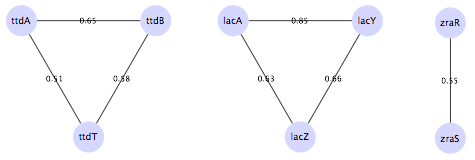
\includegraphics[scale=2]{images/Clusters-GCN_Ecoli} \centering
\caption{Clusters selected from gene co-expression network.}
\label{fig:mod_GCN-1} 
\end{figure}

\subsection*{Bayesian learning}

Clusters showed in Figure \ref{fig:mod_GCN-1} are the input for Bayesian learning but before we must discretize its expression values with the \textquotedblleft discretize\textquotedblright{} function in the \textquotedblleft bnlearn\textquotedblright{} package of R. See \cite{Nagarajan:2013:BNR:2487420}. Later, we execute three simulations of 1000 iterations, one per cluster, and we obtain the following results:
\begin{figure}
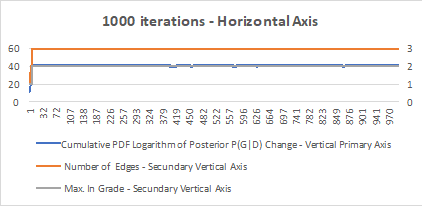
\includegraphics[scale=2.5]{images/sim1000-lac_Ecoli} \centering
\caption{Simulation of 1000 iterations for lacA, lacY and lacZ genes.}
\label{fig:sim_lac-1} 
\end{figure}
\begin{figure}
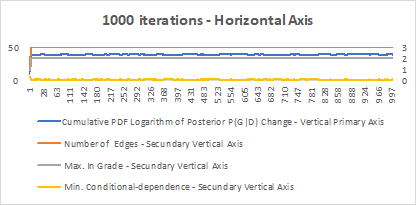
\includegraphics[scale=2.5]{images/sim1000-ttd_Ecoli} \centering
\caption{Simulation of 1000 iterations for ttdA, ttdB and ttdT genes.}
\label{fig:sim_ttd-2} 
\end{figure}
\begin{figure}
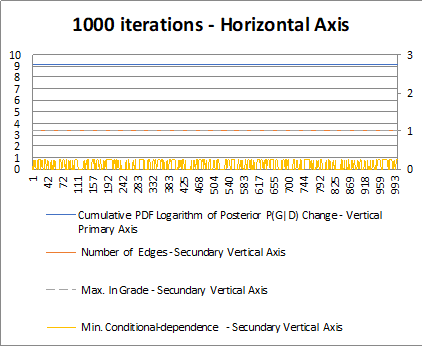
\includegraphics[scale=2.5]{images/sim1000-zra_Ecoli} \centering
\caption{Simulation of 1000 iterations for zraR and zraS genes.}
\label{fig:sim_zra-3} 
\end{figure}
We can see in the figures of above that optimal level of the density function posterior to the data is achieved during the firsts iterations in all simulations. Also, we can observe that the number of edges and the maximum in-grade are constant during simulations.\\
\\
In summary, we obtained 6 different Bayesian networks in the first and second simulation and 2 Bayesian networks in third simulation.

\subsection*{Weighted network}

In previous sub-section, we obtained several Bayesian networks as result of learning process. Now we take the sub-set of networks and averaging each edge over total of networks obtained, we get a weighted network per simulation. The result is shown to continuation: 
\begin{figure}
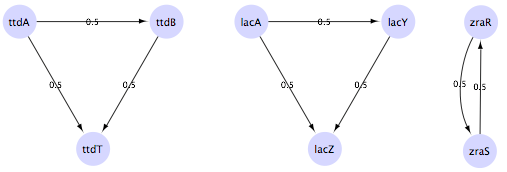
\includegraphics[scale=2.5]{images/wn-40-34-52_Ecoli} \centering
\caption{Weighted networks learned corresponding to modules 40, 34 and 52 of E. coli.}
\label{fig:wn_40-34-52} 
\end{figure}

\section*{Discussion}

\subsection*{Relation between co-expression network and Bayesian network}

We can observe in table \ref{fig:mod_GCN-1} that co-expressed genes inside each cluster also it present dependence relations between them, as it is shown in figure \ref{fig:wn_40-34-52}. If we see this from point of view mathematics seems logic that two variables whose values present high correlation, also it shows conditional dependence, talking probabilistically, i.e. these results are an effect numeric and no biological. May be this the reason because from Bayesian paradigm of statistics is not enough for to predict other bacterial regulatory system component like regulators or basal machinery if not there are high numeric correlation between them from expression data. In conclusion, we recommend articulate other machine learning approaches to complement this paradigm and achieve better predictions. 

\subsection*{Trend to overfitting when we try select more than one cluster}

Other observation is trend to overfitting in the Bayesian learning process. For instance, we try adding other component (lacI regulator gene) in the simulation of the lacA, lacY and lacZ genes and we saw the addition of edges from lacI to each modular gene. The figure \ref{fig:wn_34-lacI} shows the weighted network of the simulation. 
\begin{figure}
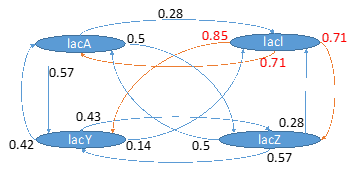
\includegraphics[scale=2.5]{images/wn-34-lacI_Ecoli} \centering
\caption{Weighted network of module 34 after of adding lacI regulator gene.}
\label{fig:wn_34-lacI} 
\end{figure}
The same effect is observed when adding rpoD and znuA genes (see figure
\ref{fig:wn_34-rpoD-znuA}).
\begin{figure}
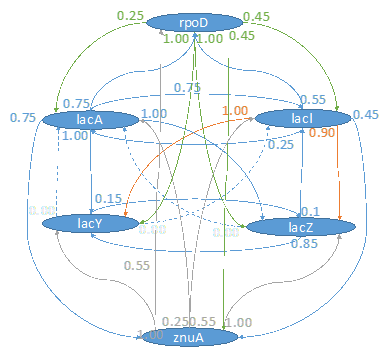
\includegraphics[scale=2.5]{images/wn-34-rpoD-znuA_Ecoli} \centering
\caption{Weighted network of module 34 after adding rpoD and znuA genes.}
\label{fig:wn_34-rpoD-znuA} 
\end{figure}
Overfitting can become chronic if we include more than one cluster in one simulation. The figure \ref{fig:wn_overfit} shows this situation.
\begin{figure}
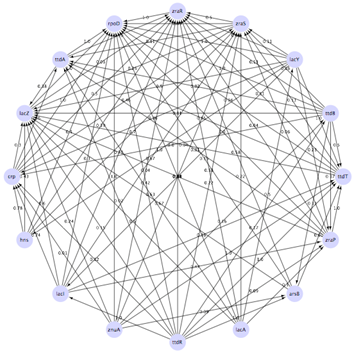
\includegraphics[scale=2.5]{images/wn-overfit_Ecoli} \centering
\caption{Trend to overfitting when several clusters are included inside one
MCMC simulation.}
\label{fig:wn_overfit} 
\end{figure}
In conclusion, we recommend highly to apply Bayesian learning process only to clusters of gene co-expression networks to avoid overfitting of Bayesian networks. 

\section*{Conclusions and future work}
\begin{itemize}
\item We found Bayesian networks that correspond to some components of modular genes like Lactose in Escherichia coli, among others. Predictions was successfully confirmed with respect to gene interactions published.
\item We see that Bayesian networks can help us to understand some bacterial regulatory systems components, mainly components of modular genes, however, its learning method only from microarray gene expression data cannot say us something about other components such as global regulators, inter-modular regulators or basal machinery.
\item A future work may be analyzing possibility of articulate Bayesian learning with other learning approaches like network science, neural networks, fractal analysis, contact maps or dependences networks (based on constraints) to do prediction of other bacterial regulatory system components. 
\end{itemize}
\pagebreak
%%%%%%%%%%%%%%%%%%%%%%%%%%%%%%%%%%%%%%%%%%%%%%
%%                                          %%
%% Backmatter begins here                   %%
%%                                          %%
%%%%%%%%%%%%%%%%%%%%%%%%%%%%%%%%%%%%%%%%%%%%%%

\begin{backmatter}

%\section*{Competing interests}
%  The authors declare that they have no competing interests.

%\section*{Author's contributions}
%    Text for this section \ldots

\section*{Acknowledgements}
  Proffesors: Rafael Tovar (Universidad del Valle), Jorge Finke(Universidad Javeriana), Pedro Moreno (Universidad del Valle) and Julio Freyre (UNAM).
%%%%%%%%%%%%%%%%%%%%%%%%%%%%%%%%%%%%%%%%%%%%%%%%%%%%%%%%%%%%%
%%                  The Bibliography                       %%
%%                                                         %%
%%  Bmc_mathpys.bst  will be used to                       %%
%%  create a .BBL file for submission.                     %%
%%  After submission of the .TEX file,                     %%
%%  you will be prompted to submit your .BBL file.         %%
%%                                                         %%
%%                                                         %%
%%  Note that the displayed Bibliography will not          %%
%%  necessarily be rendered by Latex exactly as specified  %%
%%  in the online Instructions for Authors.                %%
%%                                                         %%
%%%%%%%%%%%%%%%%%%%%%%%%%%%%%%%%%%%%%%%%%%%%%%%%%%%%%%%%%%%%%


% if your bibliography is in bibtex format, use those commands:
\bibliographystyle{bmc-mathphys} % Style BST file (bmc-mathphys, vancouver, spbasic).
\bibliography{bmc_article}      % Bibliography file (usually '*.bib' )
% for author-year bibliography (bmc-mathphys or spbasic)
% a) write to bib file (bmc-mathphys only)
% @settings{label, options="nameyear"}
% b) uncomment next line
%\nocite{label}

% or include bibliography directly:
% \begin{thebibliography}
% \bibitem{b1}
% \end{thebibliography}

%%%%%%%%%%%%%%%%%%%%%%%%%%%%%%%%%%%
%%                               %%
%% Figures                       %%
%%                               %%
%% NB: this is for captions and  %%
%% Titles. All graphics must be  %%
%% submitted separately and NOT  %%
%% included in the Tex document  %%
%%                               %%
%%%%%%%%%%%%%%%%%%%%%%%%%%%%%%%%%%%

%%
%% Do not use \listoffigures as most will included as separate files

%\section*{Figures}
%  \begin{figure}[h!]
%  \caption{\csentence{Sample figure title.}
%      A short description of the figure content
%      should go here.}
%      \end{figure}
%
%\begin{figure}[h!]
%  \caption{\csentence{Sample figure title.}
%      Figure legend text.}
%      \end{figure}

%%%%%%%%%%%%%%%%%%%%%%%%%%%%%%%%%%%
%%                               %%
%% Tables                        %%
%%                               %%
%%%%%%%%%%%%%%%%%%%%%%%%%%%%%%%%%%%

%% Use of \listoftables is discouraged.
%%


%%%%%%%%%%%%%%%%%%%%%%%%%%%%%%%%%%%
%%                               %%
%% Additional Files              %%
%%                               %%
%%%%%%%%%%%%%%%%%%%%%%%%%%%%%%%%%%%

\end{backmatter}
\end{document}
